\section{Vorlesung 11.11.2016}
\subsection{Ohrenzerlegung}

Es sei nur dann ein Graph \textit{G(V,E)} mit $|E|>=2$, der 2-Vertex-verbunden ist, gegeben, wenn es eine offene Ohrenzerlegung gibt. Jede Ohrenzerlegeung definiere eine Kreisbasis. \textcolor{red}{Kreisbasis oder Ohrenbasis???}

\begin{figure}[htp]
\centering
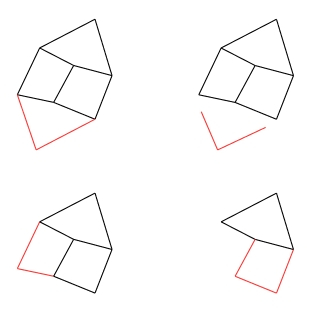
\includegraphics[scale=1.00]{lectures/161111/pix/pic1.jpg}
\end{figure}

\begin{itemize}
	\item \textbf{\textit{Kreisbasis:}} \newline Ein Ohr Sei ein maximaler Pfad P, $|P| >= 1$, so dass P nur an Endpunkten Kanten aus $E\notin P$ berührt. Die Knoten in P, die keine Endknoten sind haben immer Grad $deg = 2$.
	\item \textbf{\textit{offene Ohrenzerlegung}}\newline Eine Folge von Ohren $P_1, P_2, ..., P_k$ ist eine offene Ohrenzerlegung, wenn $P_1$ ein Kreis, $P_k$ und alle anderen $P_i$ Ohren in $G_i = G_{i+1} \setminus P_{i+1}$
\end{itemize}

\newpage
\subsubsection{Algorithmus der Ohrenzerlegung}
\begin{enumerate}
	\item Finde \textcolor{red}{Spannbaum T} für G und wähle eine Wurzel\\
		\begin{figure}[htp]
		\centering
		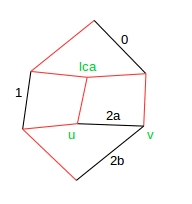
\includegraphics[scale=1.00]{lectures/161111/pix/pic2.jpg}
		\end{figure}
	\item Für jede Kante (u,v), die nicht Teil des Spannbaums ist (0,1,2a,2b), finde den \textit{\textcolor{green}{lowest common ancestor (lca)}} der Knoten u und v.
	\item Fuer jede Kante (u,v) soll die Hauptkante (w,x) gefunden werden, wobei (u,v) und (w,x) Teil eines Kreises sind und (w,x) einen \textit{lowest common ancestor} so nah wie moeglich an der Wurzel haben und (w,x) $\notin$ von T ist.
	\item Für alle (w,x) die nicht aus dem Spannbaum sind, trenne alle Kanten mit gleichem Wert ab. Diese Kanten bilden ein Ohr.
	\item Ordne die Ohren nach ihrem Gewicht. 
\end{enumerate}

\newpage
\subsection{Unabhängigkeitssysteme und Matroide}

Viele \textit{Greedy Probleme} lassen sich mittels Matroiden beschreiben (insbesondere Graphenprobleme).

\begin{itemize}
	\item \textbf{\textit{Unabhängigkeitssystem:}} \newline Ein Unabhängigkeitssystem ist ein Paar $M = (S,l)$ mit endlicher Menge $S$ und $l <= P_S(S)$ (Powerset von S). Es besitzt folgende Eigenschaften:
	\begin{itemize}
		\item[\underline{M1:}] $\emptyset = \{\} \in l$ $\rightarrow$ Die leere Menge ist unabhängig
		\item[\underline{M2:}] $x \subseteq Y \in l \rightarrow x \in l$ (Erblichkeitseigenschaft)
	\end{itemize}
	Die Elemente $x \in l$ heißen unabhängig, die Elemente $z \in P_S(S) \setminus l$ heißen abhängig. \newline
	$\rightarrow$ Kostenfunktion C: S $\rightarrow \mathbb{R}$ 
	\item \textbf{\textit{Austauscheigenschaft:}}
	\begin{itemize}
		\item [\underline{M3:}] Falls $A \in l, B \in l, |A| < |B|$, dann $\exists x, x \in B \setminus A: A \cup \{x\} \in l$
	\end{itemize}
\end{itemize}

\subsubsection{Matroid}
\begin{itemize}
	\item[] Ein Unabhängigkeitssystem sei ein Matroid falls die Eigenschaften eines Unabhängigkeitssystems und die Austauscheigenschaft erfüllt sind.
	\item[] \textit{grafischer Matroid}\newline Ein graphischer Matroid $M_G = (S_G,l_G)$ mit $S_G = E(G)$
	\begin{itemize}
		\item[$\rightarrow$] für $A \subseteq S_G: \in l_G \leftrightarrow$ A ist kein Kreis
		\item[$\rightarrow$] Menge an Kanten ist nur dann unabhängig, wenn G' = (V(G),A) einen Wald bilden $\rightarrow$ G' bildet keinen Kreis
	\end{itemize}
\end{itemize}

\underline{\textit{Extension:}} \newline Sei M = (S,l) und x $\notin$ A gegeben, so sei l eine Erweiterung von A, falls $A \cup \{x\}$ unabhängig ist. ($A \cup \{x\}\in l$) \newline  $\rightarrow$ Kante l ist eine Erweiterung, falls $A \cup \{x\}$ keinen Kreis bilden. \newline 

\underline{\textit{Maximalität:}} $A \in l$ ist maximal, falls es keine Erweiterung für A gibt. \newline

\textbf{Theorem} \newline Alle maximal unabhängigen Teilmengen in einem Matroid haben die selbe Größe.
\\\\
\textbf{Beweis} \newline Wenn das Theorem nicht gilt, so wären die maximal unabhängigen Elemente A und B mit $|A| < |B|$. Damit würde M3 zeigen, dass x abhängig von A ist: $\exists\ x: B\setminus A: A \cup \{x\}$. $\rightarrow$ \underline{Beweis durch Widerspruch}
\\\\
\textbf{Beispiel}\newline Gegeben Graph G gilt, dass alle Spannbäume, die gleiche Anzahl an Kanten haben: $|E| = |V| - 1$. \newline
\begin{itemize}
	\item \textbf{\textit{gewichtetes Matroid}} \newline Ein Matroid M=(S,l) ist gewichtet, falls es eine Gewichtsfunktion\\$w(x) > 0\ \forall\ x \in S$ gibt. $\rightarrow$ w(A), A $\subseteq$ S mit w(A) = $\displaystyle \sum_{x \in A} w(x)$.
\end{itemize}

\subsubsection{Greedy Algorithmen auf Matroiden}

Gegeben sei M(S,l). Finde $A \in l$, sodass w(A) maximal ist.\newline

\textbf{Beispiel:} Minimallänge Spannbäume mit \newline $w'(x) 0 w_0 - w(x)$ mit $w_0 = max_{x}(w(x)) + \epsilon$ \newline

\textbf{\textit{Greedy-Algorithmus}}
\begin{itemize}
	\item[1] $A \leftarrow \{ \}$
	\item[2] sortiere S[M] nach absteigendem Gewicht
	\item[3] $\forall x \in S[M] \{$ if $A\cup \{x\} \in l$: then A $\leftarrow A \cup \{x\}\}$
	\item[4] return A
\end{itemize}

\textbf{Theorem} \newline A ist die optimale Lösung des Greedy-Algorithmus \newline

\textbf{Beispiel: minimal lange Kreisbasen}\\
Betrachte und bilde Kreisbasen L1 oder L2.\\
\begin{figure}[htp]
\centering
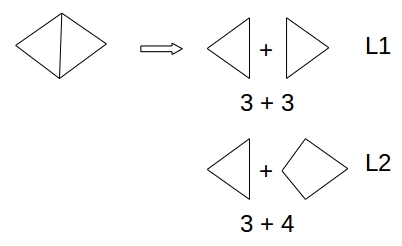
\includegraphics[scale=1.00]{lectures/161111/pix/pic3.jpg}
\end{figure}
L1 hat insgesamt weniger Knoten als L2 und ist somit eine bessere Lösung. C(G) ist ein Matroid mit den Elementgewichten $|C| \rightarrow$ diese definieren S $\rightarrow$ die minimalen Kreisbasen werden in polynomieller Zeit in $|C|$ berechnet.
\subsubsection{Horton-Algorithmus (1972)}
\begin{itemize}
	\item[1]Konstruiere die kürzesten Pfadbäume mittels Matroide. 
	\item[2]Extrahiere die fundamentalen/minimalen Kreise der Pfadbäume.
\end{itemize}
$\rightarrow$ Berechnung ist polynomiell abhängig von $|V|$
\begin{itemize}
	\item essentielle Kreise sind Kreise, die in allen minimalen Kreisbasen vorkommen. 
	\item relevante Kreise sind Kreise, die in mindestens einer minimalen Kreisbasenlösung vorkommen.
	\item Falls C nicht in ein einfacher Kreis ist, dann ist C keine minimale Kreisbase.
\end{itemize}